\documentclass[conference]{IEEEtran}

\usepackage{cite}
\usepackage[pdftex]{color}
\usepackage[pdftex]{graphicx}
%\usepackage[cmex10]{amsmath}
%\usepackage{algorithmic}
\usepackage{alltt}
\usepackage{url}
\usepackage{xspace}

\usepackage{my}

\begin{document}

\title{SimSoC-CERT: \\ a Certified Simulator for Systems on Chip}

%\author{\IEEEauthorblockN{Xxx Yyy}
%\IEEEauthorblockA{Zzz}}

\author{\IEEEauthorblockN{F. Blanqui, C. Helmstetter, V. Joloboff, J.-F. Monin, X. Shi}
\IEEEauthorblockA{INRIA, CNRS \& Tsinghua University}}

\maketitle

\begin{abstract}
The design and debugging of Systems-on-Chip
using a hardware implementation is difficult
and requires heavy material.
\emph{Simulation} is an interesting alternative approach,
which is both more flexible and less expensive.
SimSoC~\cite{ossc09} is a fast instruction set simulator
for various ARM, PowerPC, and RISC-based
architectures.
However, speed involves tricky short-comings and design decisions,
resulting in a complex software product.
This makes the accuracy of the simulator a non-trivial question:
%and the reliability of the output of simulations a relevant problem:
there is a strong need to strengthen the confidence that
%what is simulated corresponds exactly to the future hardware. => WRONG: TLM models are not cycle accurate
simulations results match the expected accuracy. % replacement of previous line
We therefore decided to \emph{certify} SimSoC, that is,
to formally prove in Coq the correctness of a significant part of this software.
% en quoi ecrire du coq certifie du C/C++ ?
The present paper reports our first efforts in this direction,
targeting the ARMv6 architecture.
% JF: Je vire car il y a plus à dire (simlight, tests) et pas de place
% We already formalized in Coq the ARMv6 architecture
% where the most tedious parts were automatically derived
% from the reference manual.

\end{abstract}

%%%%%%%%%%%%%%%%%%%%%%%%%%%%%%%%%%%%%%%%%%%%%%%%%%%%%%%%%%%%%%%%%%%%%%%%%%%%%
\section{Introduction}

\subsection{Simulation of Systems-on-Chip}

Systems-on-Chip (SoC), used in devices such as smartphones, contain both
hardware and software. A part of the software is generic and can be used with
any hardware systems, and thus can be developed on any computer. In contrast,
developing and testing the SoC-specific code can be done only with this SoC, or
with a {\em software executable model} of the SoC. To reduce the time-to-market,
the software development must start before the hardware is ready. Even if the
hardware is available, simulating the software on a model provides more
debugging capabilities.

% Using the hardware description (RTL) as a model for software
% simulation is not a good idea  % TODO: find a better expression?
The hardware description (RTL) is not a good model for software simulation
because RTL simulations are too slow
compared to the real speed of the SoC. Writing a model that can be used
as a fast simulator requires to abstract details. Thus, a functional
simulator describes the functionality of the hardware, ignoring all
the hardware features whose aim is only to speed up the computations
(e.g., cache, pipe-line,$\ldots$).

The most abstract and fastest simulators use native simulation. The
software of the {\em target} system (i.e., the SoC) is compiled with
the normal compiler of the computer running the simulator (latter
called the {\em host} machine), but linked with special system
libraries. Examples of such simulators are the Android and iOS
SDKs.
% [JF: Keep the following for long version]
% Native simulators make it possible to develop applications containing
% specific system calls, but only architecture-independent code (in
% particular, no assembly code).

In order to develop low-level system code, one needs a simulator that
can take the real binary code as input. Such a simulator requires a
model of the processor and of its peripherals (such as UART, DMA,
Ethernet card, etc). When simulating a smartphone SoC, this kind of
functional simulators can be from 1 to 10 times slower than the real
chip.
%
These simulators have other uses, for example, as
reference models for the hardware verification.
An error in the simulator can then mislead both the software and the hardware
engineers.
QEMU~\cite{qemu} is an open-source processor emulator
coming with a set of device models; it can simulate several % a variety of
operating systems. Other open-source simulators include
UNISIM~\cite{unisim} (accurately-timed)
and
SimSoC~\cite{ossc09} -- the basis of the work reported here --
which is loosely-timed (thus faster).
Simics~\cite{simics} is a commercial alternative.
%
The usual language to develop such simulators is C++, combined with
the SystemC~\cite{systemc-lrm} and OSCI-TLM~\cite{tlm-osci}
libraries.
% [JF: Keep the following for long version]
% [hope that the reader appreciates the complexity without it]
% The SystemC library, which is defined by an IEEE norm,
% provides classes to ease the description of hardware.
% Each hardware component is described by a SystemC {\em module}; modules are
% connected by SystemC {\em channels} (possibly defined in the OSCI-TLM
% library). Each module can contains one or many {threads}, which
% are {scheduled} by the SystemC kernel.

\subsection{The need for Certification}

Altogether,
a functional simulator is a complex piece of software. SimSoC, which is
able to simulate Linux both on ARM and PowerPC architectures at a realistic speed,
includes about 60,000 lines of C++ code. The code uses complex features of the
C++ language and of the SystemC library. Moreover, achieving high
simulation speeds requires complex optimizations, such as dynamic
translation~\cite{qemu}.

This complexity is problematic,  because beyond speed,
\emph{accuracy} is required:
all instructions have to be simulated
exactly as described in the documentation.
There is a strong need to strengthen the confidence that
%what is simulated corresponds exactly to the future hardware. => WRONG: TLM models are not cycle accurate
simulations results match the expected accuracy. % replacement of previous line
Intensive tests are a first answer.
For instance, as SimSoC is able to run a Linux kernel
on top of a simulated ARM, we know that many situations are covered.
However it turned out, through further experiments, that it was not
sufficient: wrong behaviors coming from rare instructions
were observed after several months.

Therefore we propose here to \emph{certify} the simulator,
that is, to prove, using \emph{formal methods} --
here: the Coq proof assistant \cite{Coqmanual, coqart} --
that it conforms to the expected behavior.
In theory, this would mean to provide a mathematical description
of the whole software and prove correctness % and completeness
properties about it.
This task is beyond our available manpower.
We then decided to focus our efforts on a sensible component of the
system: the CPU part of the ARMv6 architecture (used by the ARM11 processor family).

This corresponds to a specific component of the SimSoC simulator,
which was previously implementing only the ARMv5 instruction set.
Rather than certifying this component, it seemed to us more feasible
to design a new one directly in C, in such a way that it can be
executed alone, or integrated in SimSoC (by including the C code in
the existing C++ code).
%
% Frama-C combined with Coq targets the
% certification of C code, but not C++ code. Certifying an existing component would have
% required to extract it from SimSoC and then to translate it to C. It is more
% realistic to write a new module
%
We call this new component \simlight. Combined with a small {\tt main} function,
\simlight can simulates ARMv6 programs as long as they do not access any
peripherals (excepted the physical memory) nor coprocessors. There is no MMU
yet. Integrating it in SimSoC just requires to replace the memory interface and to
connect the interrupts (IRQ and FIQ) signals.

The present paper reports our first efforts in this direction.
% to formalize the part of SimSoC related to the simulation of an ARM processor.
We already have a formal description of the ARMv6 architecture,
where the most tedious parts was automatically derived
from the reference manual.
Indeed, \simlight was derived using a similar process.
We are now in the way of exploiting these results for
generating massive tests, with a significant and controllable coverage
of the instruction set,
and then for performing correctness proofs.

\begin{figure}
\scalebox{.5}{\insertfig{archi}}
\caption{Overall Architecture}
\label{fig:archi}
\end{figure}

Fig.~\ref{fig:archi} describes the overall architecture. The current
contributions of the work presented in this paper are the formal specification
and the simulator of the ARMv6 instruction set. The main ongoing task is to
prove the equivalence of these two items.

% RELATED WORK (to be put elsewhere?)

\emph{Related Work.}
A fully manual formalization of the ARM architecture (v7) is reported
in \cite{FoxM10}.  The formal framework is HOL4 instead of Coq, and no
specific target is considered, whereas we are driven by the needs of
simulation of ARMv6 and are secured by the automatic generation
of code and formulas described in Section \ref{sec:autogen}.

The rest of the paper is organized as follows.
Section \ref{sec:coq} provides a brief overview of Coq.
%the proof-assistant used in SimSoC-CERT.
Section \ref{sec:sc}, the core of the paper, gives the design
principles of SimSoC-CERT as well as some technical illustrations.
We conclude in section \ref{sec:concl} with some hints on
our current research directions.



%\subsection{Overall Architecture} % A.3 => Claude
% (cf. subsection~\ref{ss:proof}) % [now in the conclusion]
%%%%%%%%%%%%%%%%%%%%%%%%%%%%%%%%%%%%%%%%%%%%%%%%%%%%%%%%%%%%%%%%%%%%%%%%%%%%%
\section{Coq} % B => Jean-Francois
\label{sec:coq}

\subsection{A proof assistant}

Thorough introductions to Coq can be found in \cite{Coqmanual, coqart}.
Here we give only general principles,
%a very brief overview and of the Coq language.
informal explanations will come along with examples
in the rest of the paper.

Coq is an interactive proof-assistant:
users provide definitions, theorem statements,
and commands for interactively building proofs.
The system helps to fill easy proof steps
(propositional tautologies for instance or, at a more advanced level,
Prolog-like first-order reasoning or additive arithmetic) but
in general, creative steps, such as finding a good invariant
or a suitable witness for proving an existential statement,
require imagination and human intervention.
In any case, the main added-value of Coq is provided by its
\emph{proof-checker}, which checks that every deduction step
conforms to well-known and carefully designed logical rules.
The proof-checker is often called the kernel of the system.
Its size is reasonably small (a couple of thousands lines of code)
and is considered as extremely reliable.

Coq allows the user to formally describe a system using a combination
of mathematical (or logical) definitions.
The simplest objects are
well-known data structures such as Booleans, natural numbers,
tuples, records, lists or trees.
Next we can define functions on these objects using case analysis
and recursion.
In other words, Coq embeds a purely functional programming language.
Data structures and functions are uniformly considered as
mathematical values, on which we can reason with usual
mathematical techniques: equational reasoning, induction, etc.
For instance it is easy to define the state of an arbitrary
digital system, using tuples or records with appropriate fields.
A memory is better represented as a function from $A$
to \textit{word}, where $A$ represents the space of addresses
and \textit{word} tuples of bits of appropriate size, typically 32.
All these objects are typed according to a rich typing system
which goes far beyond the limitations of usual programming languages.

After formally describing a system, one can state
conjectures expressing that it behaves
as expected, and try to prove them.
The Coq language includes logical connectives and quantifiers,
and proofs are build interactively using deduction rules
\`a la Gentzen. % (TODO ref to UFM).

Coq has been successfully used in several applications
in computer science
such as multiplier circuits \cite{Pau95},
concurrent communication protocols \cite{EG96}, self-stabilizing
population protocols \cite{DM09}, devices for broadband protocols
\cite{Mon98}, compilers \cite{Ler06},
as well as in mathematics, e.g.\ a fully formal proof of
the 4-color theorem \cite{Gon07}.

%%%%%%%%%%%%%%%%%%%%%%%%%%%%%%%%%%%%%%%%%%%%%%%%%%%%%%%%%%%%%%%%%%%%%%%%%%%%%
\section{SimSoC-CERT} % C => Xiaomu
\label{sec:sc}

In this section, we present how we obtained the Coq formal specification of
the ARMv6 instruction set from the original but informal specification
given in the Architecture Reference Manual, part~A.
%
In this manual, each instruction is
introduced by its 32 bits encoding field, the instruction syntax, the
pseudo-code describing its behavior, and other notes on usage. The textual
English parts have been encoded in Coq by hand, but we built generators for the
other parts.

% The semi-formal pseudo-code is the basis of
% expressing instruction in a program language.


\subsection{Data-structures Representing the Processor State}

For basic data types, such as 32-bits vectors, we reused the definitions of the
CompCert project \cite{lerbla08, lerCACM09}.
The types come with additional functions (e.g., shifts and bitwise operations)
and proved properties.

We defined a data structure called \emph{state}, which stores the current global
state of the ARM system. The global state contains the state of the processor,
including its registers, and the state of the memory.
The behavior of the system is defined by the possible changes of this state.

In addition of the types, we implemented  accessor functions and
mutator functions (i.e., functions returning a new state, since Coq functions
have no side effects). These functions are used in the formal description
of the instructions.

An instruction is formalized as a mathematical function which takes
the current global state as input and returns either a new state (including a new
value for the PC), or a special value representing an {\em ``unpredictable''} state
in the reference manual terminology.

\subsection{Primitive Functions}

The definition of an instruction may use primitive functions.
For example, the {\tt B} instruction mentions a function called \emph{SignExtend\_30},
whose meaning is:
``sign-extend (propagate the sign bit) of the 24 bits argument to 30 bits''.
%, and the function called \emph{Logical\_Shift\_Left}.
Most of these functions are
described in the glossary of the ARM reference manual.
However, these descriptions use natural language, which cannot be
automatically encoded into Coq or any other language. Fortunately, there
are not many of them, and the functions are clearly expressed. We have implemented
them in Coq by hand.

\subsection{Translation of Instructions}
% Then it is neccessary to present the instruction set in SimSoC-Cert.

The example described by Fig.~\ref{ex1} shows the operation pseudo-code of the
{\tt B} instruction (Branch) .% which causes a branch to a computed target address.
The {\tt B} instruction is conditional and may optionally store the return address in the
link register {\tt LR}.

\begin{figure}[h]
\small
\begin{alltt}
if ConditionPassed(cond) then
    if L == 1 then
        LR = address of the instruction
             after the branch instruction
    PC = PC+(SignExtend_30(signed_immed_24)<<2)
\end{alltt}
\caption{Instruction BL in ARM ref. manual pseudo-code}\label{ex1}
\end{figure}

Our main target language is Coq. The way to express an instruction in
Coq is illustrated in Fig.~\ref{ex2}.
The instruction operation is defined in Coq with monadic specifications~\cite{wadjfp09},
in order to express changes of internal states
in a readable way
and to facilitate the reasoning on the intermediate computations.
%whether the operation is sequential or parallel.

For a Coq specification, it is necessary to define the
semantics in Coq of all the pseudo-code constructs, such as conditional and assignment statements.
The general \emph{if\ldots then\ldots else} construct of Coq is purely functional:
a value has to be returned in all cases, which means that
the two branches \emph{then} and \emph{else} have to be considered.
In our case, it is more convenient to provide special constructs
to be used for translating operations involving an \emph{if\_then} branch,
%where the silent \emph{else} branch leads to an ``unpredictable'' state. % WRONG !!!!!!!!!!!!!!!!!!!!!!
where the silent \emph{else} branch returns an unmodified state. % please confirm this version
%For other statement like \emph{loop}, \emph{sequential} need to be defined too.

\begin{figure}
\small
\begin{alltt}
Definition B_step (s0 : state) (L : bool)
    (cond : opcode)
    (signed_immed_24 : word) : result :=
  if_then (ConditionPassed s0 cond)
    (block (
      if_then (zeq L 1)
        (set_reg LR
           (address_of_next_instruction s0))::
      set_reg PC (add (reg_content s0 PC)
        (Logical_Shift_Left
          (SignExtend_30 signed_immed_24)
          (repr 2)))::
      nil)) true s0.
\end{alltt}
\caption{Instruction BL in Coq}\label{ex2}
\end{figure}

We also formalized the decoding of instructions.
The relevant information is presented in a 32 bits encoding field,
like the one in Fig.~\ref{encode}.
We go back to this in the following section. % So why do we talk of this now?

\begin{figure}
\hfil \begin{tabular}{|c|ccc|c|c|}
\hline
31 .. 28 & 27 & 26 & 25 & 24 &  23 \dotfill 0  \\
\hline
  cond   & 1  & 0  & 1  & L  & signed\_immed\_24\\
\hline
\end{tabular}
\caption{The BL instruction encoding}
\label{encode}
\end{figure}

\subsection{An Automatic Generator}
\label{sec:autogen}

The reference manual contains pseudo-code for the 148 instructions
of the ARM, as well as for the 36 addressing modes
and for exception handling operations.
Manually translating these pieces of pseudo-code is a tedious and error-prone task.
Therefore, we built a software tool which automatically
generates the Coq description from the reference pseudo-code.
In Fig.\ref{step}, the architecture of the generator is presented. The path on the
left shows the automatic generation flow from the reference manual to Coq
specifications.
The pseudo-code is extracted from a text version of the reference manual
and parsed to an abstract syntax tree (AST).
Then, code is generated for the Coq specification.
% and also for \simlight (in C++).
Building the analyzers allowed us to detect a dozen of mistakes
in the reference manual (including misspelling and missing code), which we submitted to the ARM company.
At the moment, the rectifications are gathered in a patch file.
The same idea (and some code) is reused to generate massive tests
for SimSoC (right branch on Fig.\ref{step}).

\begin{figure}
\centering
% 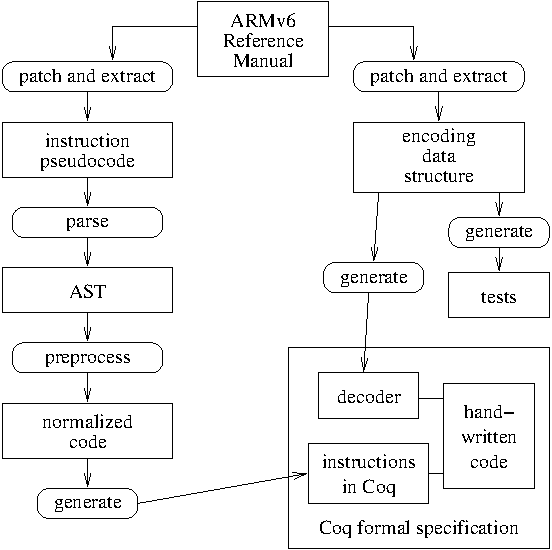
\includegraphics[scale=0.8]{generationStep.png}
\scalebox{.8}{\insertfig{generationStep}}
\caption{The automatic generation steps}
\label{step}
\end{figure}

The reliability of this process comes from two considerations:
first, we could check on different kinds of instructions that
the generated code is as expected;
and second, the impact of a mistake in the generator ranges over
many (if not all) instructions, which would make it easy to detect.
Moreover, Fig.\ref{fig} shows that the generator is much smaller than
the generated code.

\begin{figure}
\hfil \begin{tabular}{|l|r@{ }l|}
\hline
code generator & 9096 & words \\
generated instructions & 21457 & words \\
generated decoder & 9709 & words \\
hand-written Coq & 9120 & words \\
\hline
\end{tabular}
\caption{Figures of code generation}
\label{fig}
\end{figure}

% TODO: give number of lines too

% Note: figures for the generator should exclude genpc, gencxx, and gentest
%                                (+ validity.ml because it is not used yet)


The middle path in Fig.~\ref{step} represents the automatic generation step for a Coq
decoder. The data structure is extracted from the instruction encoding field; it
is a list containing a 32 bits array for each instruction and each addressing
mode. Each element of the array describes the kind of the bit: the bit can be
fixed to 0 or 1, or be part of an instruction parameter.
For the {\tt B} instruction (see Fig.~\ref{encode}), bits 27 to 25 are fixed,
and all others give the value of the parameters (cond, L, and
signed\_immed\_24).  Moreover, some instructions have
\emph{``should be zero/one''} bits,
meaning that the instruction is unpredictable if the bit does not have this value.

The generated {\tt decode} function uses a large pattern-matching. Each pattern
is a sequence of 0, 1, and jokers for any bits which are not fixed.  This large
pattern-matching has to be carefully ordered because of potential redundancies.
For example, any instruction starting with the bits {\tt 1111101...} matches the
encoding array of the {\tt B} instruction, but is not a {\tt B} instruction
because {\tt 1111} is not a valid value for the ``cond'' field.  Consequently,
unconditional instructions (bits 31 to 28 fixed to {\tt 1111}) need to be
considered before conditional ones. In the general case, if many instructions
can match the same binary word, then they must be ordered decreasingly according to
their number of fixed-bits. Note that a wrong order raises a Coq compiler error
(because a pattern is detected as unreachable), not a runtime error.

% \begin{figure}
% \begin{tabular}{|c|c|c|c|}
% \hline
% Code generator & Generated instr. & Generated decoder
% & hand written\\
% \hline
% 9096 words&21457 words&9709 words&9120 words\\
% \hline
% \end{tabular}
% \caption{Figu  res of code generation}
% \label{fig-obso}
% \end{figure}

%From the figures, we can say this automatic generator makes more efficiency and less trouble.

% [Claude] I do understand the paragraph below. Looks like it is self-contradictory.
% So I've removed it, but you are welcome to add it again if you can fix it.

% And the coverage of instruction transformation is high,
% it can reach one hundred percent. It means all the
% ARM instructions included in ARMv6 can be transformed. The 'while'
% statement is not defined yet. Currently tests do not use those
% instruction, this will be fix later.


\subsection{Test generation}

% [Claude] Make clear this is an ongoing work (less than
% 10% done), on the contrary of the remaining of this section.

Starting from the encoding tables extracted from the reference manual and used
to generate the decoder, we can generate massive binary tests.
This test generator is now based on random generation.
First, the test generator selects one instruction. Next, for the fixed bits it
generates the corresponding values; and for the parameters it generates a random
value.
It can generate both valid instructions and \emph{unpredictable} instructions.

We are continuing to develop this test generator in order to generate tests in a
more systematic way: we plan to generate all combinations of enumerated and
Boolean parameters. For immediate values, we will select the bounds and a few
random values.
The expected result (i.e., the assembly code) has to be generated at the same
time than the binary word, in order to automatize the result checking.

With these binary instructions, we can test SimSoC, thus increasing our
confidence in SimSoC. The generated tests have already been useful to design and
validate the decoder of \simlight.



% We expect to have all the possible cases and all the \emph{unpredictable}
% cases. % [Claude] Are you sure? it makes 2^32 !

% This can be achieved by filling the variables and significant bits using
% all the valid combinations or the combinations leading to an \emph{unpredictable}
% instruction.

%after we can have a
%percentage of correctness of SimSoC decoder.

%%%%%%%%%%%%%%%%%%%%%%%%%%%%%%%%%%%%%%%%%%%%%%%%%%%%%%%%%%%%%%%%%%%%%%%%%%%%%
\section{Conclusion}
\label{sec:concl}

%{Ongoing Work}

We have presented how we have obtained a formal specification of the CPU part of
the ARMv6 architecture. In the same way, we have written the \simlight
simulator.  This simulator has been obtained using the same architecture: 85~\%
of its code is generated from the reference manual, with only 860 lines added to
the generators. We have tested \simlight both with the generated and the
existing SimSoC tests.

One work to do in the future is to complete the test generator.
On the other hand, we started to state and prove some properties about the primitive
functions, in order to improve our confidence in their hand-written specifications.
Next, the core work is to build a proof of the correctness of \simlight, using the
Coq formalization as the reference specification.
% by proving the pre-condition and post-condition of a piece of
% program in \simlight is equivalent to the one in Coq specification.

At least, to complete the Coq specifications, we may introduce the system-control
coprocessor and MMU models into SimSoC-CERT. As other parts of the manual are
mainly written in English, this task would have to be done by hand.

% {Equivalence Proof}

% TODO: we must prove that the \simlight code is equivalent to the Coq specification.




%%%%%%%%%%%%%%%%%%%%%%%%%%%%%%%%%%%%%%%%%%%%%%%%%%%%%%%%%%%%%%%%%%%%%%%%%%%%%
\bibliographystyle{IEEEtran}
\bibliography{cert}

\end{document}
